\subsection{Initial value}
%
We begin by encoding $\counterstart$ with the Seed unit.
%
It has $\ceil*{\frac{d}{3}}$ digit regions.
%
Each digit region has three digits, except for the most significant digit region (MSR) which has $d \mod 3$ if $d \mod 3 \not= 0$, otherwise it has 3 digits.
%

\begin{figure}[H]
    \centering
    \subcaptionbox{MSR case 1\label{fig:initial_case1_msr}}{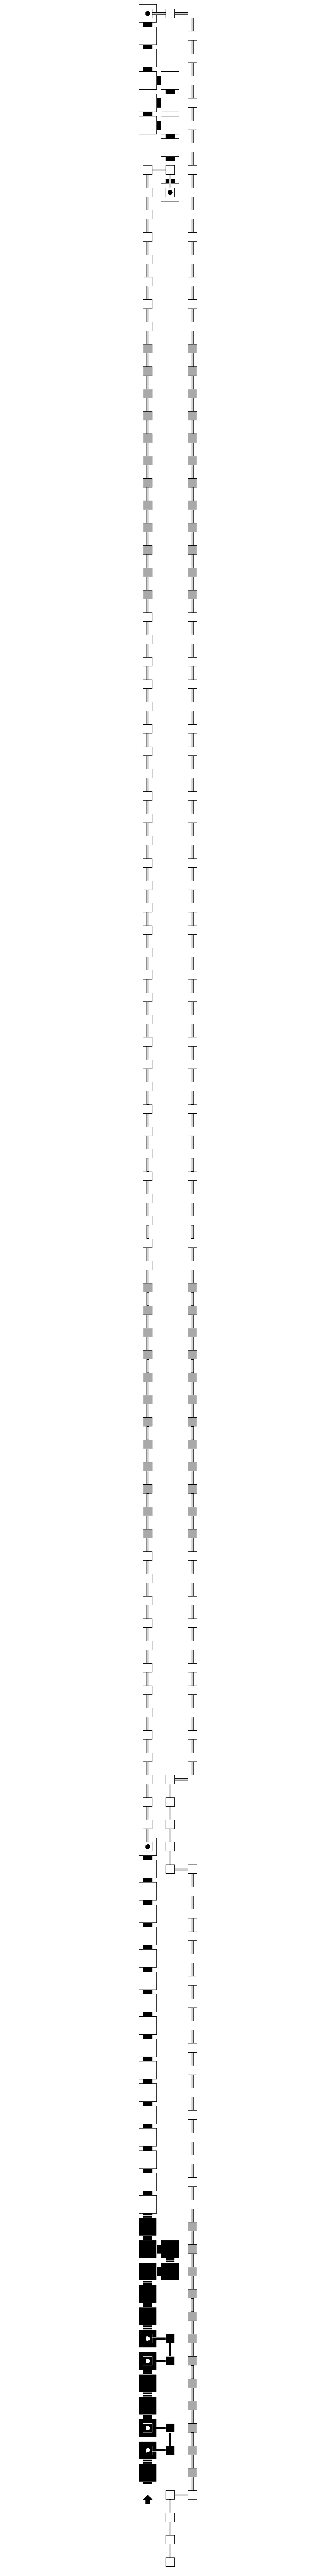
\includegraphics[width=0.95in]{initial_value_case_1_msr}}\hfill%
    \subcaptionbox{MSR case 2\label{fig:initial_case2_msr}}{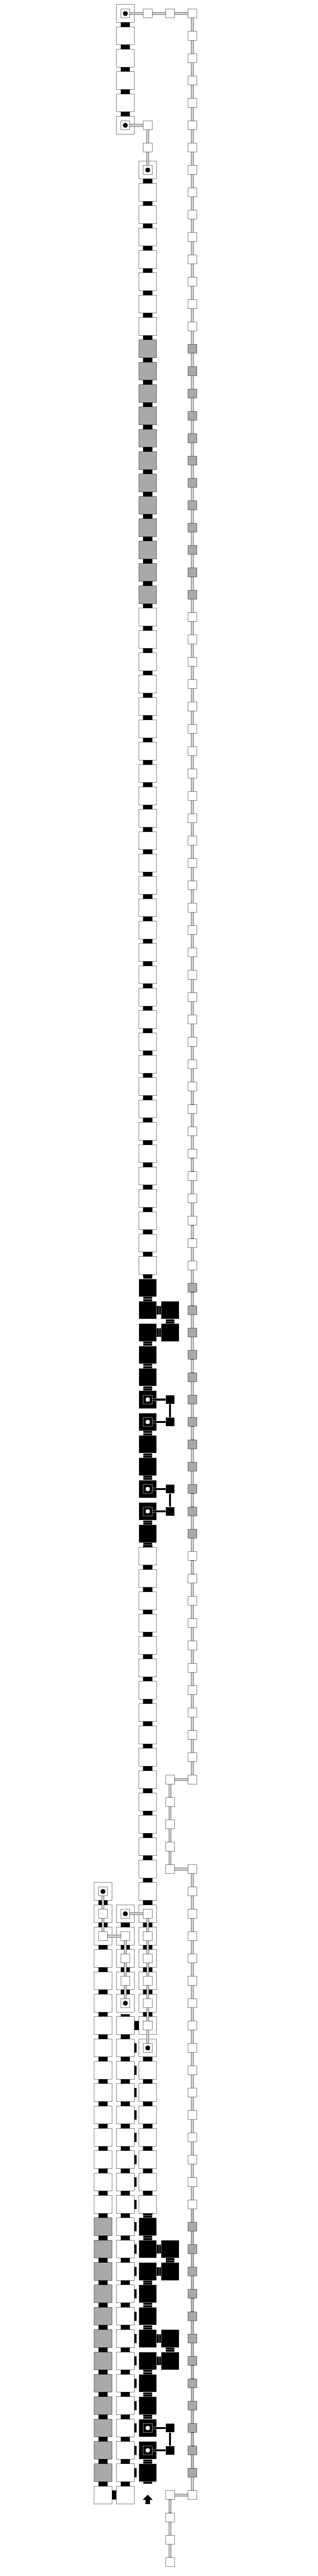
\includegraphics[width=0.95in]{initial_value_case_2_msr}}\hfill%
    \subcaptionbox{MSR case 3\label{fig:initial_case3_msr}}{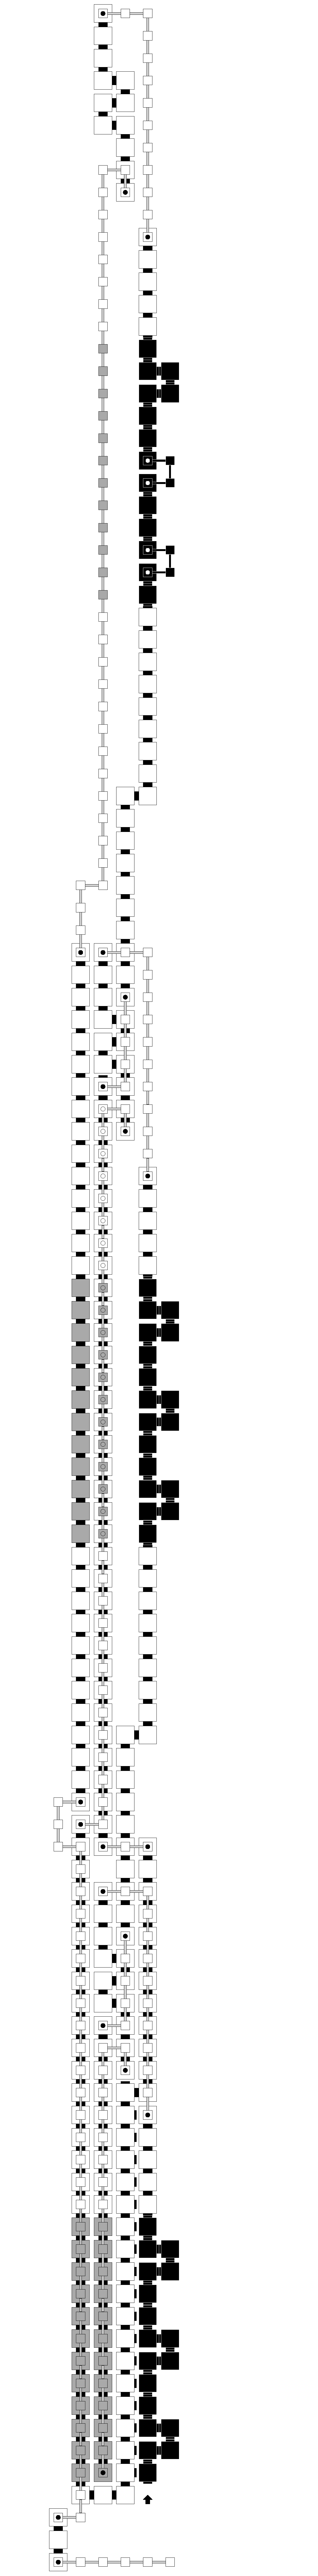
\includegraphics[width=0.95in]{initial_value_case_3_msr}}\hfill%
    \subcaptionbox{General digit regions\label{fig:initial_general}}{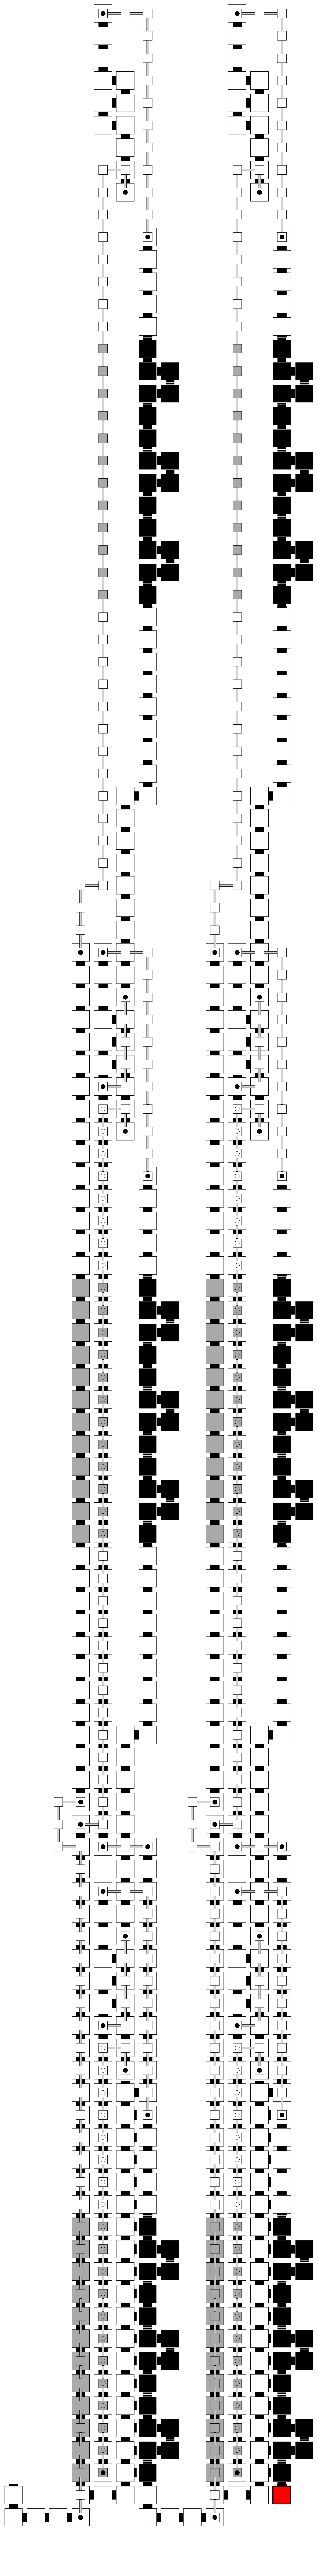
\includegraphics[width=0.95in]{initial_value_general}}%
    \caption{\label{fig:initial_value_assemblies} These figures show an example construction of the initial value,
    with all the possible MSR to the left. Of the three possible MSRs, of course only one would occur in a real assembly.}
\end{figure}

Note that we use $i$ as the index of a digit in $\counterstart$ and $j$ as the index of a bit
in a encoded digit.

\begin{itemize}
    \item Create
    $\begin{aligned}[t]
        {\tt Seed}(&\left\langle {\tt CounterWrite}, 1, {\tt seed}, 0, 0 \right\rangle \; )
    \end{aligned}$
\end{itemize}


The idea here is to repeat these steps starting from $i = 0$ and repeating until $i$ is the index of the first digit in the MSR. These
steps build general non-MSR digit regions shown in Figure~\ref{fig:initial_general}.


\subsubsection{General}
For $i = 0,\dots,3g$:
\begin{itemize}
    \item {\tt Start}.

    \item {\tt Digit}, for each $j=0,\ldots,l-1$ and each $b$ in $bin(s[i])[j]$:
    \begin{itemize}
        \item if $j = 0$:\\ create
        $\begin{aligned}[t]
            \cwrite(&\left\langle {\tt CounterWrite}, 1, {\tt seed}, i, j \right\rangle, \left\langle {\tt CounterWrite}, 1, {\tt seed}, i, j + 1 \right\rangle \;)
        \end{aligned}$\\from the general gadget shown in Figure~\ref{fig:counter_write_0}.

        \item if $j = 1$:\\ create
        $\begin{aligned}[t]
            \cwrite(&\left\langle {\tt CounterWrite}, 1, {\tt seed}, i, j \right\rangle, \left\langle {\tt CounterWrite}, 1, {\tt seed}, i, j + 1 \right\rangle \;)
        \end{aligned}$\\from the general gadget shown in Figure~\ref{fig:counter_write_0}.

        \item if $1 < j < l-1$:\\ create
        $\begin{aligned}[t]
            \cwrite(&\left\langle {\tt CounterWrite}, 1, {\tt seed}, i, j \right\rangle, \left\langle {\tt CounterWrite}, 1, {\tt seed}, i, j + 1 \right\rangle \;)
        \end{aligned}$\\from the general gadget shown in Figure~\ref{fig:counter_write_0} if $b = 0$ or Figure~\ref{fig:counter_write_1} if $b = 1$.

        \item if $j = l-1$: create
        $\begin{aligned}[t]
            \cwrite(&\left\langle {\tt CounterWrite}, 1, {\tt seed}, i, j \right\rangle, \left\langle {\tt DigitTop}, 1, {\tt seed}, i \right\rangle \;)
        \end{aligned}$\\from the general gadget shown in Figure~\ref{fig:counter_write_0} if $b = 0$ or Figure~\ref{fig:counter_write_1} if $b = 1$.
    \end{itemize}
    %
    In this step, assuming the maximum of 8 tiles are used for each bit $b$, then
    %
    $\sum^{l-1}_{j=0} 8 = 8l =$
    %
    $8 \cdot \left( \ceil*{\log m} + 2 \right) \leq$
    %
    $8 \cdot \left( {\log m} + 3 \right) =$
    %
    $8 \cdot {\log m} + 24$ tiles were created.
    %

    \item {\dtop}, the following statements create the gadget shown in Figure~\ref{fig:digit_top_general}.
    \begin{itemize}
        \item Create
        $\begin{aligned}[t]
            {\tt North\_Line5}(& \left \langle {\tt DigitTop},  1, {\tt seed}, i \right\rangle,
                                 \left \langle {\tt DigitTopA}, 1, {\tt seed}, i \right\rangle \;)
        \end{aligned}$\\ from the micro-gadget shown in Figure~\ref{fig:north_line}.

        \item Create
        $\begin{aligned}[t]
            {\tt Topper}(& \left\langle {\tt DigitTopA}, 1, {\tt seed}, i \right\rangle,
                           \left\langle {\tt DigitTopB}, 1, {\tt seed}, i \right\rangle \;)
        \end{aligned}$\\ from the micro-gadget shown in Figure~\ref{fig:topper_gen}.

        \item Create
        $\begin{aligned}[t]
            {\tt South\_Line4\textit{l}}(& \left\langle {\tt DigitTopB},  1, {\tt seed}, i\right\rangle,
                                           \left\langle {\tt ReturnPath}, 1, {\tt seed}, i\right\rangle \;)
        \end{aligned}$\\ from the micro-gadget shown in Figure~\ref{fig:south_line}.
    \end{itemize}
    %
    In this step, $40 + 4l =$
    %
    $40 + 4 \cdot \left( \ceil*{\log m} + 2 \right) \leq$
    %
    $40 + 4 \cdot \left( {\log m} + 3 \right) =$
    %
    $52 + 4 \cdot {\log m}$ tiles were created.
    %

    \item Create
    $\begin{aligned}[t]
            \returnpath(&\left\langle {\tt ReturnPath}, 1, {\tt seed}, i \right\rangle,
                         \left\langle {\tt NextRead},   1, {\tt seed}, i \right\rangle \;)
    \end{aligned}$\\ (single tile).
    %
    In this step, $1$ tile was created.
    %

    \item $i \gets i + 1$.

    \item Create
    $\begin{aligned}[t]
            \nextread(&\left\langle {\tt NextRead},   1, {\tt seed}, i - 1\right\rangle,
                       \left\langle {\tt SecondWarp}, 2, {\tt seed}, i    \right\rangle \;)
    \end{aligned}$\\ (single tile).
    %
    In this step, $1$ tile was created.
    %

    \item Create
    $\begin{aligned}[t]
        \secondwarp(&\left\langle {\tt SecondWarp}, 2, {\tt seed}, i \right\rangle,
                     \left\langle {\tt PostWarp},   2, {\tt seed}, i \right\rangle \;)
    \end{aligned}$ (single tile).
    %
    In this step, $1$ tile was created.
    %

    \item Create
    $\begin{aligned}[t]
        \postwarp(&\left\langle {\tt PostWarp},     2, {\tt seed}, i    \right\rangle,
                   \left\langle {\tt CounterWrite}, 2, {\tt seed}, i, 0 \right\rangle \;)
    \end{aligned}$\\ from the general gadget show in Figure~\ref{fig:post_warp_2or3_op}.
    %
    In this step, $25$ tiles were created.
    %

    \item {\tt Digit}: for each $j=0,\ldots,l-1$, where $b$ is $bin(s[i])[j]$:
    \begin{itemize}
        \item if $j = 0$:\\ create
        $\begin{aligned}[t]
            \cwrite(&\left\langle {\tt CounterWrite}, 2, {\tt seed}, i, j \right\rangle, \left\langle {\tt CounterWrite}, 2, {\tt seed}, i, j + 1 \right\rangle \;)
        \end{aligned}$\\from the general gadget shown in Figure~\ref{fig:counter_write_0}.

        \item if $j = 1$:\\ create
        $\begin{aligned}[t]
            \cwrite(&\left\langle {\tt CounterWrite}, 2, {\tt seed}, i, j \right\rangle, \left\langle {\tt CounterWrite}, 2, {\tt seed}, i, j + 1 \right\rangle \;)
        \end{aligned}$\\from the general gadget shown in Figure~\ref{fig:counter_write_0}.

        \item if $1 < j < l-1$:\\ create
        $\begin{aligned}[t]
            \cwrite(&\left\langle {\tt CounterWrite}, 2, {\tt seed}, i, j \right\rangle, \left\langle {\tt CounterWrite}, 2, {\tt seed}, i, j + 1 \right\rangle \;)
        \end{aligned}$\\from the general gadget shown in Figure~\ref{fig:counter_write_0} if $b = 0$ or Figure~\ref{fig:counter_write_1} if $b = 1$.

        \item if $j = l-1$: create
        $\begin{aligned}[t]
            \cwrite(&\left\langle {\tt CounterWrite}, 2, {\tt seed}, i, j \right\rangle, \left\langle {\tt DigitTop}, 2, {\tt seed}, i \right\rangle \;)
        \end{aligned}$\\from the general gadget shown in Figure~\ref{fig:counter_write_0} if $b = 0$ or Figure~\ref{fig:counter_write_1} if $b = 1$.
    \end{itemize}
    %
    In this step, assuming the maximum of 8 tiles are used for each bit $b$, then
    %
    $\sum^{l-1}_{j=0} 8 = 8l =$
    %
    $8 \cdot \left( \ceil*{\log m} + 2 \right) \leq$
    %
    $8 \cdot \left( {\log m} + 3 \right) =$
    %
    $8 \cdot {\log m} + 24$ tiles were created.
    %

    \item {\dtop}: the following statements create the gadget shown in Figure~\ref{fig:digit_top_general}.
    \begin{itemize}
        \item Create
        $\begin{aligned}[t]
            {\tt North\_Line5}(& \left \langle {\tt DigitTop},  2, {\tt seed}, i \right\rangle,
                                 \left \langle {\tt DigitTopA}, 2, {\tt seed}, i \right\rangle \;)
        \end{aligned}$\\ from the micro-gadget shown in Figure~\ref{fig:north_line}.

        \item Create
        $\begin{aligned}[t]
            {\tt Topper}(& \left \langle {\tt DigitTopA}, 2, {\tt seed}, i \right\rangle,
                           \left \langle {\tt DigitTopB}, 2, {\tt seed}, i \right\rangle \;)
        \end{aligned}$\\ from the micro-gadget shown in Figure~\ref{fig:topper_gen}.

        \item Create
        $\begin{aligned}[t]
            {\tt South\_Line4\textit{l}}(&\left\langle {\tt DigitTopB},  2, {\tt seed}, i \right\rangle,
                                          \left\langle {\tt ReturnPath}, 2, {\tt seed}, i \right\rangle \;)
        \end{aligned}$\\ from the micro-gadget shown in Figure~\ref{fig:south_line}.
    \end{itemize}
    %
    In this step, $40 + 4l =$
    %
    $40 + 4 \cdot \left( \ceil*{\log m} + 2 \right) \leq$
    %
    $40 + 4 \cdot \left( {\log m} + 3 \right) =$
    %
    $52 + 4 \cdot {\log m}$ tiles were created.
    %

    \item Create
    $\begin{aligned}[t]
        \returnpath(&\left\langle {\tt ReturnPath}, 2, {\tt seed}, i \right\rangle,
                     \left\langle {\tt NextRead},   2, {\tt seed}, i \right\rangle \;)
    \end{aligned}$\\ from the gadget in Figure~\ref{fig:return_path_2_op-or-seed}.
    %
    In this step, $32 + 4l$ tiles were created.
    %

    \item $i \gets i + 1$.

    \item Create
    $\begin{aligned}[t]
        \nextread(&\left\langle {\tt NextRead},  2, {\tt seed}, i - 1 \right\rangle,
                   \left\langle {\tt FirstWarp}, 3, {\tt seed}, i     \right\rangle \;)
    \end{aligned}$\\ from the general gadget shown in Figure~\ref{fig:next_read_2_seed_op}.
    %
    In this step, $3$ tiles were created.
    %

    \item Create
    $\begin{aligned}[t]
        \firstwarp(&\left\langle {\tt FirstWarp},  3, {\tt seed}, i \right\rangle,
                    \left\langle {\tt WarpBridge}, 3, {\tt seed}, i \right\rangle \;)
    \end{aligned}$ (single tile).
    %
    In this step, $1$ tile was created.
    %

    \item Create
    $\begin{aligned}[t]
        \warpbridge(&\left\langle {\tt WarpBridge}, 3, {\tt seed}, i \right\rangle,
                     \left\langle {\tt SecondWarp}, 3, {\tt seed}, i \right\rangle \;)
    \end{aligned}$\\ from the general gadget shown in Figure~\ref{fig:warp_bridge_general}.
    %
    In this step, $29$ tiles were created.
    %

    \item Create
    $\begin{aligned}[t]
        \secondwarp(&\left\langle {\tt SecondWarp}, 3, {\tt seed}, i  \right\rangle,
                     \left\langle {\tt PostWarp},   3, {\tt seed}, i  \right\rangle \;)
    \end{aligned}$ (single tile).
    %
    In this step, $1$ tile was created.
    %

    \item Create
    $\begin{aligned}[t]
        \postwarp(&\left\langle {\tt PostWarp},     3, {\tt seed}, i    \right\rangle,
                   \left\langle {\tt CounterWrite}, 3, {\tt seed}, i, 0 \right\rangle \;)
    \end{aligned}$\\from the general gadget shown in Figure~\ref{fig:post_warp_2or3_op}.
    %
    In this step, $25$ tiles were created.
    %

    \item {\tt Digit}: for each $j=0,\ldots,l-1$ and each $b$ in $bin(s[i])[j]$:
    \begin{itemize}
        \item if $j = 0$:\\ create
        $\begin{aligned}[t]
            \cwrite(&\left\langle {\tt CounterWrite}, 3, {\tt seed}, i, j \right\rangle, \left\langle {\tt CounterWrite}, 3, {\tt seed}, i, j + 1 \right\rangle \;)
        \end{aligned}$\\from the general gadget shown in Figure~\ref{fig:counter_write_0}.

        \item if $j = 1$:\\ create
        $\begin{aligned}[t]
            \cwrite(&\left\langle {\tt CounterWrite}, 3, {\tt seed}, i, j \right\rangle, \left\langle {\tt CounterWrite}, 3, {\tt seed}, i, j + 1 \right\rangle \;)
        \end{aligned}$\\from the general gadget shown in Figure~\ref{fig:counter_write_0}.

        \item if $1 < j < l-1$:\\ create
        $\begin{aligned}[t]
            \cwrite(&\left\langle {\tt CounterWrite}, 3, {\tt seed}, i, j \right\rangle, \left\langle {\tt CounterWrite}, 3, {\tt seed}, i, j + 1 \right\rangle \;)
        \end{aligned}$\\from the general gadget shown in Figure~\ref{fig:counter_write_0} if $b = 0$ or Figure~\ref{fig:counter_write_1} if $b = 1$.

        \item if $j = l-1$: create
        $\begin{aligned}[t]
            \cwrite(&\left\langle {\tt CounterWrite}, 3, {\tt seed}, i, j \right\rangle, \left\langle {\tt DigitTop}, 3, {\tt seed}, i \right\rangle \;)
        \end{aligned}$\\from the general gadget shown in Figure~\ref{fig:counter_write_0} if $b = 0$ or Figure~\ref{fig:counter_write_1} if $b = 1$.
    \end{itemize}
    %
    In this step, assuming the maximum of 8 tiles are used for each bit $b$, then
    %
    $\sum^{l-1}_{j=0} 8 = 8l =$
    %
    $8 \cdot \left( \ceil*{\log m} + 2 \right) \leq$
    %
    $8 \cdot \left( {\log m} + 3 \right) =$
    %
    $8 \cdot {\log m} + 24$ tiles were created.
    %

    \item {\dtop}, the following statements create the gadget shown in Figure~\ref{fig:digit_top_general}.
    \begin{itemize}
        \item Create
        $\begin{aligned}[t]
            {\tt North\_Line5}(&\left\langle {\tt DigitTop},  3, {\tt seed}, i \right\rangle,
                                \left\langle {\tt DigitTopA}, 3, {\tt seed}, i \right\rangle \;)
        \end{aligned}$\\from the micro-gadget shown in Figure~\ref{fig:north_line}.

        \item Create
        $\begin{aligned}[t]
            {\tt Topper}(&\left\langle {\tt DigitTopA}, 3, {\tt seed}, i \right\rangle,
                          \left\langle {\tt DigitTopB}, 3, {\tt seed}, i \right\rangle \;)
        \end{aligned}$\\from the micro-gadget shown in Figure~\ref{fig:topper_gen}.

        \item Create
        $\begin{aligned}[t]
            {\tt South\_Line4\textit{l}}(&\left\langle {\tt DigitTopB},  3, {\tt seed}, i \right\rangle,
                                          \left\langle {\tt ReturnPath}, 3, {\tt seed}, i \right\rangle \;)
        \end{aligned}$\\from the micro-gadget shown in Figure~\ref{fig:south_line}.
    \end{itemize}
    %
    In this step, $40 + 4l =$
    %
    $40 + 4 \cdot \left( \ceil*{\log m} + 2 \right) \leq$
    %
    $40 + 4 \cdot \left( {\log m} + 3 \right) =$
    %
    $52 + 4 \cdot {\log m}$ tiles were created.
    %

    \item Create
    $\begin{aligned}[t]
        \returnpath(&\left\langle {\tt ReturnPath}, 3, {\tt seed}, i  \right\rangle,
                     \left\langle {\tt NextRead},   3, {\tt seed}, i, \right\rangle \;)
    \end{aligned}$\\from the gadget in Figure~\ref{fig:return_path_3}.
    %
    In this step, $65 + 8l$ tiles were created.
    %

    \item $i \gets i + 1$.

    \item Create
    $\begin{aligned}[t]
        \nextread(&\left\langle {\tt NextRead},     3, {\tt seed}, i - 1 \right\rangle,
                   \left\langle {\tt CounterWrite}, 1, {\tt seed}, i, 0  \right\rangle \;)
    \end{aligned}$\\ from the general gadget shown in Figure~\ref{fig:next_read_3_seed_op}.
    %
    In this step, $7$ tiles were created.
    %

    \item if $i$ is not an index in the MSR, go to {\tt start}, else break.
\end{itemize}

%
In this step, $\sum^{3g}_{i = 0} 311 + 48l = (3g + 1) + (48l + 311) = O\left( dl \right)$ tiles were created.
%
This means that
\begin{align*}
    dl &= O\left( d \hspace{0.1cm} {\log m} \right) \\
       &= O\left( d \hspace{0.1cm} {\log \ceil*{\left(\frac{N}{102}\right)^{\frac{1}{d}}}} \right) \\
       &= O \left(d \hspace{0.1cm} {\log \left( 2 \left( \frac{N}{102} \right)^{ \frac{1}{d} } \right) } \right) \\
       &= O \left(d \hspace{0.1cm} {\log \left( \frac{N}{102} \right)^{ \frac{1}{d} } }  + d \hspace{0.1cm} {\log 2} \right) \\
       &= O \left(d \hspace{0.1cm} {\log N} + d  \floor*{\frac{k}{2} } \right) \\
       &= O \left(\hspace{0.1cm} {\log N} \right) \\
\end{align*}
tiles were created in this step.
%


\subsubsection{Case 1}
%
If $d - i = 1$ to create the assembly shown in~\ref{fig:initial_case1_msr}.
%
\begin{itemize}
    \item {\tt Digit}, for each $j=0,\ldots,l-1$ and each $b$ in $bin(s[i])[j]$:
    \begin{itemize}
        \item if $j = 0$:\\ create
        $\begin{aligned}[t]
            \cwrite(&\left\langle {\tt CounterWrite}, 1, {\tt seed}, i, j \right\rangle, \left\langle {\tt CounterWrite}, 1, {\tt seed}, i, j + 1 \right\rangle \;)
        \end{aligned}$\\from the general gadget shown in Figure~\ref{fig:counter_write_1}.

        \item if $j = 1$:\\ create
        $\begin{aligned}[t]
            \cwrite(&\left\langle {\tt CounterWrite}, 1, {\tt seed}, i, j \right\rangle, \left\langle {\tt CounterWrite}, 1, {\tt seed}, i, j + 1 \right\rangle \;)
        \end{aligned}$\\from the general gadget shown in Figure~\ref{fig:counter_write_1}.

        \item if $1 < j < l - 1$:\\ create
        $\begin{aligned}[t]
            \cwrite(&\left\langle {\tt CounterWrite}, 1, {\tt seed}, i, j \right\rangle, \left\langle {\tt CounterWrite}, 1, {\tt seed}, i, j + 1 \right\rangle \;)
        \end{aligned}$\\from the general gadget shown in Figure~\ref{fig:counter_write_0} if $b = 0$ or Figure~\ref{fig:counter_write_1} if $b = 1$.

        \item if $j = l-1$: create
        $\begin{aligned}[t]
            \cwrite(&\left\langle {\tt CounterWrite}, 1, {\tt seed}, i, j \right\rangle, \left\langle {\tt DigitTop}, 1, {\tt seed}, i \right\rangle \;)
        \end{aligned}$\\from the general gadget shown in Figure~\ref{fig:counter_write_0} if $b = 0$ or Figure~\ref{fig:counter_write_1} if $b = 1$.
    \end{itemize}
    %
    In this step, assuming the maximum of 8 tiles are used for each bit $b$, then
    %
    $\sum^{l-1}_{j=0} 8 = 8l =$
    %
    $8 \cdot \left( \ceil*{\log m} + 2 \right) \leq$
    %
    $8 \cdot \left( {\log m} + 3 \right) =$
    %
    $8 \cdot {\log m} + 24$ tiles were created.
    %

    \item {\dtop}, the following statements create the gadget shown in Figure~\ref{fig:digit_top_1_op_msr_msd}.
    \begin{itemize}
        \item Create
        $\begin{aligned}[t]
            {\tt North\_Line4\textit{l}}(& \left\langle {\tt DigitTop},  1, {\tt seed}, i \right\rangle,
                                           \left\langle {\tt DigitTopA}, 1, {\tt seed}, i \right\rangle \;)
        \end{aligned}$\\from the micro-gadget shown in Figure~\ref{fig:north_line}.

        \item Create $\begin{aligned}[t]
            {\tt North\_Line4}(& \left\langle {\tt DigitTopA}, 1, {\tt seed}, i \right\rangle,
                                 \left\langle {\tt DigitTopB}, 1, {\tt seed}, i \right\rangle \;)
        \end{aligned}$\\from the micro-gadget shown in Figure~\ref{fig:north_line}.

        \item Create $\begin{aligned}[t]
            {\tt Topper}(& \left\langle {\tt DigitTopB}, 1, {\tt seed}, i \right\rangle,
                           \left\langle {\tt DigitTopC}, 1, {\tt seed}, i \right\rangle \;)
        \end{aligned}$\\from the micro-gadget shown in Figure~\ref{fig:topper_gen}.

        \item Create
        $\begin{aligned}[t]
            {\tt South\_Line4\textit{l}}(& \left\langle {\tt DigitTopC}, 1, {\tt seed}, i \right\rangle,
                                           \left\langle {\tt DigitTopD}, 1, {\tt seed}, i \right\rangle \;)
        \end{aligned}$\\from the micro-gadget shown in Figure~\ref{fig:south_line}.

        \item Create
        $\begin{aligned}[t]
            {\tt South\_Line30}(& \left\langle {\tt DigitTopD}, 1, {\tt seed}, i \right\rangle,
                                  \left\langle {\tt DigitTopE}, 1, {\tt seed}, i \right\rangle \;)
        \end{aligned}$\\from the micro-gadget shown in Figure~\ref{fig:south_line}.

        \item Create
        $\begin{aligned}[t]
            {\tt South\_Line4\textit{l}}(& \left\langle {\tt DigitTopE}, 1, {\tt seed}, i \right\rangle,
                                           \left\langle {\tt DigitTopF}, 1, {\tt seed}, i \right\rangle \;)
        \end{aligned}$\\ from the micro-gadget shown in Figure~\ref{fig:south_line}.

        \item Create
        $\begin{aligned}[t]
            {\tt South\_Line14}(& \left\langle {\tt DigitTopF}, 1, {\tt seed}, i\right\rangle,
                                  \left\langle {\tt DigitTopG}, 1, {\tt seed}, i\right\rangle \;)
        \end{aligned}$\\ from the micro-gadget shown in Figure~\ref{fig:south_line}.

        \item Create
        $\begin{aligned}[t]
            {\tt South\_Line17}(& \left\langle {\tt DigitTopG},  1, {\tt seed}, i \right\rangle,
                                  \left\langle {\tt ReturnPath}, 1, {\tt seed}, i  \right\rangle \;)
        \end{aligned}$\\from the micro-gadget shown in Figure~\ref{fig:south_line}.
    \end{itemize}
    %
    In this step, $100 + 12l=$
    %
    $100 + 12 \cdot \left( \ceil*{\log m} + 2 \right) \leq$
    %
    $100 + 12 \cdot \left( {\log m} + 3 \right) =$
    %
    $136 + 36 \cdot {\log m}$ tiles were created.
    %

    \item Create
    $\begin{aligned}[t]
            \returnpath(&\left\langle {\tt ReturnPath}, 1, {\tt seed}, i \right\rangle,
                         \left\langle {\tt NextRead},   1, {\tt seed}, i \right\rangle \;)
    \end{aligned}$\\from the general gadget shown in Figure~\ref{fig:return_path_1-or-2_op_msr_msd}.
    %
    In this step, $30 + 4l$ tiles were created.
    %

    \item Create
    $\begin{aligned}[t]
        \nextread(& \left\langle {\tt NextRead}, 1,      {\tt seed}, i  \right\rangle,
                    \left\langle {\tt Cross\_Next\_Row}, {\tt increment}\right\rangle \;)
    \end{aligned}$\\from the general gadget shown in Figure~\ref{fig:next_read_1-or-2_op_msr_msd}.
    %
    In this step, $37 + 4l$ tiles were created.
    %
\end{itemize}
This means that, $8l + (100 + 12l) + (30 + 4l)  + (37 + 4l) =$
$167 + 28l =$
$167 + 28 \cdot \left( \ceil*{\log m} + 2 \right) \leq $
$167 + 28 \left( {\log m} + 3 \right) =$
$O \left( {\log m} \right) $ tiles were created in this step.
%

\subsubsection{Case 2}
%
If $d - i = 2$, to create the assembly shown in~\ref{fig:initial_case2_msr}.
%
\begin{itemize}
    \item {\tt Digit}, for each $j=0,\ldots,l-1$ and each $b$ in $bin(s[i])[j]$:
    \begin{itemize}
        \item if $j = 0$:\\ create
        $\begin{aligned}[t]
            \cwrite(&\left\langle {\tt CounterWrite}, 2, {\tt seed}, i, j \right\rangle, \left\langle {\tt CounterWrite}, 2, {\tt seed}, i, j + 1 \right\rangle \;)
        \end{aligned}$\\from the general gadget shown in Figure~\ref{fig:counter_write_1}.

        \item if $j = 1$:\\ create
        $\begin{aligned}[t]
            \cwrite(&\left\langle {\tt CounterWrite}, 2, {\tt seed}, i, j \right\rangle, \left\langle {\tt CounterWrite}, 2, {\tt seed}, i, j + 1 \right\rangle \;)
        \end{aligned}$\\from the general gadget shown in Figure~\ref{fig:counter_write_0}.

        \item if $1 < j < l-1$:\\ create
        $\begin{aligned}[t]
            \cwrite(&\left\langle {\tt CounterWrite}, 2, {\tt seed}, i, j \right\rangle, \left\langle {\tt CounterWrite}, 2, {\tt seed}, i, j + 1 \right\rangle \;)
        \end{aligned}$\\from the general gadget shown in Figure~\ref{fig:counter_write_0} if $b = 0$ or Figure~\ref{fig:counter_write_1} if $b = 1$.

        \item if $j = l-1$: create
        $\begin{aligned}[t]
            \cwrite(&\left\langle {\tt CounterWrite}, 2, {\tt seed}, i, j \right\rangle, \left\langle {\tt DigitTop}, 2, {\tt seed}, i \right\rangle \;)
        \end{aligned}$\\from the general gadget shown in Figure~\ref{fig:counter_write_0} if $b = 0$ or Figure~\ref{fig:counter_write_1} if $b = 1$.
    \end{itemize}
    %
    In this step, assuming the maximum of 8 tiles are used for each bit $b$, then
    %
    $\sum^{l-1}_{j=0} 8 = 8l =$
    %
    $8 \cdot \left( \ceil*{\log m} + 2 \right) \leq$
    %
    $8 \cdot \left( {\log m} + 3 \right) =$
    %
    $8 \cdot {\log m} + 24$ tiles were created.
    %

    \item {\dtop}, the following statements create the gadget shown in Figure~\ref{fig:digit_top_1_op_msr}.
    \begin{itemize}
        \item Create
        $\begin{aligned}[t]
            {\tt Topper}(&\left\langle {\tt DigitTop},  1, {\tt seed}, i \right\rangle,
                          \left\langle {\tt DigitTopA}, 1, {\tt seed}, i \right\rangle \;)
        \end{aligned}$\\from the micro-gadget shown in Figure~\ref{fig:topper_case1}
        \item Create
        $\begin{aligned}[t]
            {\tt South\_Line4\textit{l}}(&\left\langle {\tt DigitTopA},  1, \inc, {\tt msr}\right\rangle,
                                          \left\langle {\tt ReturnPath}, 1, \inc, {\tt msr}\right\rangle \;)
        \end{aligned}$\\from the micro-gadget shown in Figure~\ref{fig:south_line}
    \end{itemize}
    %
    In this step, $43 + 4l =$
    %
    $43 + 4 \cdot \left( \ceil*{\log m} + 2 \right) \leq$
    %
    $43 + 4 \cdot \left( {\log m} + 3 \right) =$
    %
    $55 + 4 \cdot {\log m}$ tiles were created.
    %

    \item Create
    $\begin{aligned}[t]
            \returnpath(&\left\langle {\tt ReturnPath}, 1, {\tt seed}, i \right\rangle,
                         \left\langle {\tt NextRead},   1, {\tt seed}, i \right\rangle \;)
    \end{aligned}$\\ (single tile).
    %
    In this step, $1$ tile was created.
    %

    \item $i \gets i + 1$

    \item Create
    $\begin{aligned}[t]
            \nextread(&\left\langle {\tt NextRead},   1, {\tt seed}, i-1 \right\rangle,
                       \left\langle {\tt SecondWarp}, 2, {\tt seed}, i   \right\rangle \;)
    \end{aligned}$\\ (single tile).
    %
    In this step, $1$ tile was created.
    %

    \item Create
    $\begin{aligned}[t]
        \secondwarp(&\left\langle {\tt SecondWarp}, 2, {\tt seed}, i \right\rangle,
                     \left\langle {\tt PostWarp},   2, {\tt seed}, i \right\rangle \;)
    \end{aligned}$ \\ (single tile).
    %
    In this step, $1$ tile was created.
    %

    \item Create
    $\begin{aligned}[t]
        \postwarp(&\left\langle {\tt PostWarp}, 2, {\tt seed}, i    \right\rangle,
                   \left\langle {\tt CounterWrite},    2, {\tt seed}, i, 0 \right\rangle \;)
    \end{aligned}$\\ from the general gadget show in Figure~\ref{fig:post_warp_2_op_msr_msd}.
    %
    In this step, $22$ tiles were created.
    %

    \item {\tt Digit}, for each $j=0,\ldots,l-1$ and each $b$ in $bin(s[i])[j]$:
    \begin{itemize}
        \item if $j = 0$:\\ create
        $\begin{aligned}[t]
            \cwrite(&\left\langle {\tt CounterWrite}, 2, {\tt seed}, i, j \right\rangle, \left\langle {\tt CounterWrite}, 2, {\tt seed}, i, j + 1 \right\rangle \;)
        \end{aligned}$\\from the general gadget shown in Figure~\ref{fig:counter_write_1}.

        \item if $j = 1$:\\ create
        $\begin{aligned}[t]
            \cwrite(&\left\langle {\tt CounterWrite}, 2, {\tt seed}, i, j \right\rangle, \left\langle {\tt CounterWrite}, 2, {\tt seed}, i, j + 1 \right\rangle \;)
        \end{aligned}$\\from the general gadget shown in Figure~\ref{fig:counter_write_1}.

        \item if $1 < j < l-1$:\\ create
        $\begin{aligned}[t]
            \cwrite(&\left\langle {\tt CounterWrite}, 2, {\tt seed}, i, j \right\rangle, \left\langle {\tt CounterWrite}, 2, {\tt seed}, i, j + 1 \right\rangle \;)
        \end{aligned}$\\from the general gadget shown in Figure~\ref{fig:counter_write_0} if $b = 0$ or Figure~\ref{fig:counter_write_1} if $b = 1$.

        \item if $j = l-1$: create
        $\begin{aligned}[t]
            \cwrite(&\left\langle {\tt CounterWrite}, 2, {\tt seed}, i, j \right\rangle, \left\langle {\tt DigitTop}, 2, {\tt seed}, i \right\rangle \;)
        \end{aligned}$\\from the general gadget shown in Figure~\ref{fig:counter_write_0} if $b = 0$ or Figure~\ref{fig:counter_write_1} if $b = 1$.
    \end{itemize}
    %
    In this step, assuming the maximum of 8 tiles are used for each bit $b$, then
    %
    $\sum^{l-1}_{j=0} 8 = 8l =$
    %
    $8 \cdot \left( \ceil*{\log m} + 2 \right) \leq$
    %
    $8 \cdot \left( {\log m} + 3 \right) =$
    %
    $8 \cdot {\log m} + 24$ tiles were created.
    %

    \item {\dtop}, the following statements create the gadget shown in Figure~\ref{fig:digit_top_2_op_msr_msd}.
    \begin{itemize}
        \item Create
        $\begin{aligned}[t]
            {\tt North\_Line4\textit{l}}(& \left\langle {\tt DigitTop},  2, {\tt seed}, i \right\rangle,
                                           \left\langle {\tt DigitTopA}, 2, {\tt seed}, i \right\rangle\;)
        \end{aligned}$\\ from the micro-gadget shown in Figure~\ref{fig:north_line}.

        \item Create
        $\begin{aligned}[t]
            {\tt Topper}(& \left\langle {\tt DigitTopA}, 2, {\tt seed}, i \right\rangle,
                           \left\langle {\tt DigitTopB}, 2, {\tt seed}, i \right\rangle \;)
        \end{aligned}$\\from the micro-gadget shown in Figure~\ref{fig:topper_case2}.

        \item Create
        $\begin{aligned}[t]
            {\tt South\_Line4\textit{l}}(& \left\langle {\tt DigitTopB}, 2, {\tt seed}, i \right\rangle,
                                           \left\langle {\tt DigitTopC}, 2, {\tt seed}, i \right\rangle \;)
        \end{aligned}$\\from the micro-gadget shown in Figure~\ref{fig:south_line}.

        \item Create
        $\begin{aligned}[t]
            {\tt South\_Line30}(& \left\langle {\tt DigitTopC},  2, {\tt seed}, i \right\rangle,
                                  \left\langle {\tt ReturnPath}, 2, {\tt seed}, i \right\rangle \;)
        \end{aligned}$\\from the micro-gadget shown in Figure~\ref{fig:south_line}.
    \end{itemize}
    %
    In this step, $ 58 + 8l =$
    %
    $58 + 8 \cdot \left( \ceil*{\log m} + 2 \right) \leq$
    %
    $58 + 8 \cdot \left( {\log m} + 3 \right) =$
    %
    $82 + 8 \cdot {\log m}$ tiles were created.
    %

    \item Create
    $\begin{aligned}[t]
        \returnpath(& \left\langle {\tt ReturnPath}, 2, {\tt seed}, i \right\rangle,
                      \left\langle {\tt NextRead},   2, {\tt seed}, i \right\rangle \;)
    \end{aligned}$\\from the gadget shown in Figure~\ref{fig:return_path_1-or-2_op_msr_msd}.
    %
    In this step, $30 + 4l$ tiles were created.
    %

    \item Create
    $\begin{aligned}[t]
        \nextread(& \left\langle {\tt NextRead}, 2,      {\tt seed}      \right\rangle,
                    \left\langle {\tt Cross\_Next\_Row}, {\tt increment} \right\rangle \;)
    \end{aligned}$\\from the gadget shown in Figure~\ref{fig:next_read_1-or-2_op_msr_msd}.
    %
    In this step, $37 + 4l$ tiles were created.
    %
\end{itemize}
%
This means that, $8l + (43 + 4l) + 1 + 1 + 1 + 22 + 8l + (58 + 8l) + (30 + 41) + (37 + 4l) =$
%
$193 + 36l =$
%
$193 + 36 \cdot \left( \ceil*{\log m} + 2 \right) \leq $
%
$193 + 36 \left( {\log m} + 3 \right) =$
%
$O \left( {\log m} \right) $ tiles were created in this step.
%


\subsubsection{Case 3}
%
If $d - i = 3$ to create the assembly shown in~\ref{fig:initial_case3_msr}.
%
\begin{itemize}

    \item {\tt Digit}, for each $j=0,\ldots,l-1$ and each $b$ in $bin(s[i])[j]$:
    \begin{itemize}
        \item if $j = 0$:\\ create
        $\begin{aligned}[t]
            \cwrite(&\left\langle {\tt CounterWrite}, 1, {\tt seed}, i, j \right\rangle, \left\langle {\tt CounterWrite}, 1, {\tt seed}, i, j + 1 \right\rangle \;)
        \end{aligned}$\\from the general gadget shown in Figure~\ref{fig:counter_write_0}.

        \item if $j = 1$:\\ create
        $\begin{aligned}[t]
            \cwrite(&\left\langle {\tt CounterWrite}, 1, {\tt seed}, i, j \right\rangle, \left\langle {\tt CounterWrite}, 1, {\tt seed}, i, j + 1 \right\rangle \;)
        \end{aligned}$\\from the general gadget shown in Figure~\ref{fig:counter_write_0}.

        \item if $1 < j < l-1$:\\ create
        $\begin{aligned}[t]
            \cwrite(&\left\langle {\tt CounterWrite}, 1, {\tt seed}, i, j \right\rangle, \left\langle {\tt CounterWrite}, 1, {\tt seed}, i, j + 1 \right\rangle \;)
        \end{aligned}$\\from the general gadget shown in Figure~\ref{fig:counter_write_0} if $b = 0$ or Figure~\ref{fig:counter_write_1} if $b = 1$.

        \item if $j = l-1$: create
        $\begin{aligned}[t]
            \cwrite(&\left\langle {\tt CounterWrite}, 1, {\tt seed}, i, j \right\rangle, \left\langle {\tt DigitTop}, 1, {\tt seed}, i \right\rangle \;)
        \end{aligned}$\\from the general gadget shown in Figure~\ref{fig:counter_write_0} if $b = 0$ or Figure~\ref{fig:counter_write_1} if $b = 1$.
    \end{itemize}
    %
    In this step, assuming the maximum of 8 tiles are used for each bit $b$, then
    %
    $\sum^{l-1}_{j=0} 8 = 8l =$
    %
    $8 \cdot \left( \ceil*{\log m} + 2 \right) \leq$
    %
    $8 \cdot \left( {\log m} + 3 \right) =$
    %
    $8 \cdot {\log m} + 24$ tiles were created.
    %

    \item {\dtop}, the following statements create the gadget shown in Figure~\ref{fig:digit_top_general}.
    \begin{itemize}
        \item Create
        $\begin{aligned}[t]
            {\tt North\_Line5}(& \left \langle {\tt DigitTop},  1, {\tt seed}, i \right\rangle,
                                 \left \langle {\tt DigitTopA}, 1, {\tt seed}, i \right\rangle \;)
        \end{aligned}$\\ from the micro-gadget shown in Figure~\ref{fig:north_line}.

        \item Create
        $\begin{aligned}[t]
            {\tt Topper}(& \left\langle {\tt DigitTopA}, 1, {\tt seed}, i \right\rangle,
                           \left\langle {\tt DigitTopB}, 1, {\tt seed}, i \right\rangle \;)
        \end{aligned}$\\ from the micro-gadget shown in Figure~\ref{fig:topper_gen}.

        \item Create
        $\begin{aligned}[t]
            {\tt South\_Line4\textit{l}}(& \left\langle {\tt DigitTopB},  1, {\tt seed}, i\right\rangle,
                                           \left\langle {\tt ReturnPath}, 1, {\tt seed}, i\right\rangle \;)
        \end{aligned}$\\ from the micro-gadget shown in Figure~\ref{fig:south_line}.
    \end{itemize}
    %
    In this step, $40 + 4l =$
    %
    $40 + 4 \cdot \left( \ceil*{\log m} + 2 \right) \leq$
    %
    $40 + 4 \cdot \left( {\log m} + 3 \right) =$
    %
    $52 + 4 \cdot {\log m}$ tiles were created.
    %

    \item Create
    $\begin{aligned}[t]
            \returnpath(&\left\langle {\tt ReturnPath}, 1, {\tt seed}, i - 1\right\rangle,
                         \left\langle {\tt NextRead},   1, {\tt seed}, i    \right\rangle \;)
    \end{aligned}$\\ (single tile).
    %
    In this step, $1$ tile was created.
    %

    \item $i \gets i + 1$.

    \item Create
    $\begin{aligned}[t]
            \nextread(&\left\langle {\tt NextRead},   1, {\tt seed}, i - 1\right\rangle,
                       \left\langle {\tt SecondWarp}, 2, {\tt seed}, i    \right\rangle \;)
    \end{aligned}$\\ (single tile).
    %
    In this step, $1$ tile was created.
    %

    \item Create
    $\begin{aligned}[t]
        \secondwarp(&\left\langle {\tt SecondWarp}, 2, {\tt seed}, i \right\rangle,
                     \left\langle {\tt PostWarp},   2, {\tt seed}, i \right\rangle \;)
    \end{aligned}$ (single tile).
    %
    In this step, $1$ tile was created.
    %

    \item Create
    $\begin{aligned}[t]
        \postwarp(&\left\langle {\tt PostWarp}, 2, {\tt seed}, i    \right\rangle,
                   \left\langle {\tt CounterWrite},    2, {\tt seed}, i, 0 \right\rangle \;)
    \end{aligned}$\\ from the general gadget show in Figure~\ref{fig:post_warp_2or3_op}.
    %
    In this step, $25$ tiles were created.
    %

    \item {\tt Digit}, for each $j=0,\ldots,l-1$ and each $b$ in $bin(s[i])[j]$:
    \begin{itemize}
        \item if $j = 0$\\ create
        $\begin{aligned}[t]
            \cwrite(&\left\langle {\tt CounterWrite}, 2, {\tt seed}, i, j \right\rangle, \left\langle {\tt CounterWrite}, 2, {\tt seed}, i, j + 1 \right\rangle \;)
        \end{aligned}$\\from the general gadget shown in Figure~\ref{fig:counter_write_0}.

        \item if $j = 1$:\\ create
        $\begin{aligned}[t]
            \cwrite(&\left\langle {\tt CounterWrite}, 2, {\tt seed}, i, j \right\rangle, \left\langle {\tt CounterWrite}, 2, {\tt seed}, i, j + 1 \right\rangle \;)
        \end{aligned}$\\from the general gadget shown in Figure~\ref{fig:counter_write_0}.

        \item if $1 < j < l-1$:\\ create
        $\begin{aligned}[t]
            \cwrite(&\left\langle {\tt CounterWrite}, 2, {\tt seed}, i, j \right\rangle, \left\langle {\tt CounterWrite}, 2, {\tt seed}, i, j + 1 \right\rangle \;)
        \end{aligned}$\\from the general gadget shown in Figure~\ref{fig:counter_write_0} if $b = 0$ or Figure~\ref{fig:counter_write_1} if $b = 1$.

        \item if $j = l-1$: create
        $\begin{aligned}[t]
            \cwrite(&\left\langle {\tt CounterWrite}, 2, {\tt seed}, i, j \right\rangle, \left\langle {\tt DigitTop}, 2, {\tt seed}, i \right\rangle \;)
        \end{aligned}$\\from the general gadget shown in Figure~\ref{fig:counter_write_0} if $b = 0$ or Figure~\ref{fig:counter_write_1} if $b = 1$.
    \end{itemize}
    %
    In this step, assuming the maximum of 8 tiles are used for each bit $b$, then
    %
    $\sum^{l-1}_{j=0} 8 = 8l =$
    %
    $8 \cdot \left( \ceil*{\log m} + 2 \right) \leq$
    %
    $8 \cdot \left( {\log m} + 3 \right) =$
    %
    $8 \cdot {\log m} + 24$ tiles were created.
    %

    \item {\dtop}, the following statements create the gadget shown in Figure~\ref{fig:digit_top_general}.
    \begin{itemize}
        \item Create
        $\begin{aligned}[t]
            {\tt North\_Line5}(& \left \langle {\tt DigitTop},  2, {\tt seed} , i \right\rangle,
                                 \left \langle {\tt DigitTopA}, 2, {\tt seed} , i \right\rangle \;)
        \end{aligned}$\\ from the micro-gadget shown in Figure~\ref{fig:north_line}.

        \item Create
        $\begin{aligned}[t]
            {\tt Topper}(& \left \langle {\tt DigitTopA}, 2, {\tt seed}, i \right\rangle,
                           \left \langle {\tt DigitTopB}, 2, {\tt seed}, i \right\rangle \;)
        \end{aligned}$\\ from the micro-gadget shown in Figure~\ref{fig:topper_gen}.

        \item Create
        $\begin{aligned}[t]
            {\tt South\_Line4\textit{l}}(&\left\langle {\tt DigitTopB},  2, {\tt seed}, i \right\rangle,
                                          \left\langle {\tt ReturnPath}, 2, {\tt seed}, i \right\rangle \;)
        \end{aligned}$\\ from the micro-gadget shown in Figure~\ref{fig:south_line}.
    \end{itemize}
    %
    In this step, $40 + 4l =$
    %
    $40 + 4 \cdot \left( \ceil*{\log m} + 2 \right) \leq$
    %
    $40 + 4 \cdot \left( {\log m} + 3 \right) =$
    %
    $52 + 4 \cdot {\log m}$ tiles were created.
    %

    \item Create
    $\begin{aligned}[t]
        \returnpath(&\left\langle {\tt ReturnPath}, 2, {\tt seed}, i \right\rangle,
                     \left\langle {\tt NextRead},   2, {\tt seed}, i \right\rangle \;)
    \end{aligned}$\\ from the gadget in Figure~\ref{fig:return_path_2_op-or-seed}.
    %
    In this step, $32 + 4l$ tiles were created.
    %

    \item $i \gets i + 1$

    \item Create
    $\begin{aligned}[t]
        \nextread(&\left\langle {\tt NextRead},  2, {\tt seed}, i - 1 \right\rangle,
                   \left\langle {\tt FirstWarp}, 3, {\tt seed}, i     \right\rangle \;)
    \end{aligned}$\\ from the general gadget shown in Figure~\ref{fig:next_read_2_seed_op}.
    %
    In this step, $3$ tiles were created.
    %

    \item Create
    $\begin{aligned}[t]
        \firstwarp(&\left\langle {\tt FirstWarp},  3, {\tt seed}, i \right\rangle,
                    \left\langle {\tt WarpBridge}, 3, {\tt seed}, i \right\rangle \;)
    \end{aligned}$ (single tile).
    %
    In this step, $1$ tile was created.
    %

    \item Create
    $\begin{aligned}[t]
        \warpbridge(&\left\langle {\tt WarpBridge}, 3, {\tt seed}, i \right\rangle,
                     \left\langle {\tt SecondWarp}, 3, {\tt seed}, i \right\rangle \;)
    \end{aligned}$\\ from the general gadget shown in Figure~\ref{fig:warp_bridge_general}.
    %
    In this step, $29$ tiles were created.
    %

    \item Create
    $\begin{aligned}[t]
        \secondwarp(&\left\langle {\tt SecondWarp}, 3, {\tt seed}, i  \right\rangle,
                     \left\langle {\tt PostWarp},   3, {\tt seed}, i  \right\rangle \;)
    \end{aligned}$ (single tile).
    %
    In this step, $1$ tile was created.
    %

    \item Create
    $\begin{aligned}[t]
        \postwarp(&\left\langle {\tt PostWarp}, 3, {\tt seed}, i    \right\rangle,
                   \left\langle {\tt CounterWrite},    3, {\tt seed}, i, 0 \right\rangle \;)
    \end{aligned}$\\from the general gadget shown in Figure~\ref{fig:post_warp_2or3_op}.
    %
    In this step, $25$ tiles were created.
    %

    \item {\tt Digit}, for each $j=0,\ldots,l-1$ and each $b$ in $bin(s[i])[j]$:
    \begin{itemize}
        \item if $j = 0$:\\ create
        $\begin{aligned}[t]
            \cwrite(&\left\langle {\tt CounterWrite}, 3, {\tt seed}, i, j \right\rangle, \left\langle {\tt CounterWrite}, 3, {\tt seed}, i, j + 1 \right\rangle \;)
        \end{aligned}$\\from the general gadget shown in Figure~\ref{fig:counter_write_1}.

        \item if $j = 1$:\\ create
        $\begin{aligned}[t]
            \cwrite(&\left\langle {\tt CounterWrite}, 3, {\tt seed}, i, j \right\rangle, \left\langle {\tt CounterWrite}, 3, {\tt seed}, i, j + 1 \right\rangle \;)
        \end{aligned}$\\from the general gadget shown in Figure~\ref{fig:counter_write_1}.

        \item if $1 < j < l-1$:\\ create
        $\begin{aligned}[t]
            \cwrite(&\left\langle {\tt CounterWrite}, 3, {\tt seed}, i, j \right\rangle, \left\langle {\tt CounterWrite}, 3, {\tt seed}, i, j + 1 \right\rangle \;)
        \end{aligned}$\\from the general gadget shown in Figure~\ref{fig:counter_write_0} if $b = 0$ or Figure~\ref{fig:counter_write_1} if $b = 1$.

        \item if $j = l-1$: create
        $\begin{aligned}[t]
            \cwrite(&\left\langle {\tt CounterWrite}, 3, {\tt seed}, i, j \right\rangle, \left\langle {\tt DigitTop}, 3, {\tt seed}, i \right\rangle \;)
        \end{aligned}$\\from the general gadget shown in Figure~\ref{fig:counter_write_0} if $b = 0$ or Figure~\ref{fig:counter_write_1} if $b = 1$.
    \end{itemize}
    %
    In this step, assuming the maximum of 8 tiles are used for each bit $b$, then
    %
    $\sum^{l-1}_{j=0} 8 = 8l =$
    %
    $8 \cdot \left( \ceil*{\log m} + 2 \right) \leq$
    %
    $8 \cdot \left( {\log m} + 3 \right) =$
    %
    $8 \cdot {\log m} + 24$ tiles were created.
    %

    \item {\dtop}, the following statements create the gadget shown in Figure~\ref{fig:digit_top_general}.
    \begin{itemize}
        \item Create
        $\begin{aligned}[t]
            {\tt North\_Line5}(&\left\langle {\tt DigitTop},  3, {\tt seed}, i \right\rangle,
                                \left\langle {\tt DigitTopA}, 3, {\tt seed}, i \right\rangle \;)
        \end{aligned}$\\from the micro-gadget shown in Figure~\ref{fig:north_line}.

        \item Create
        $\begin{aligned}[t]
            {\tt Topper}(&\left\langle {\tt DigitTopA}, 3, {\tt seed}, i \right\rangle,
                          \left\langle {\tt DigitTopB}, 3, {\tt seed}, i \right\rangle \;)
        \end{aligned}$\\from the micro-gadget shown in Figure~\ref{fig:topper_gen}.

        \item Create
        $\begin{aligned}[t]
            {\tt South\_Line4\textit{l}}(&\left\langle {\tt DigitTopB},  3, {\tt seed}, i \right\rangle,
                                          \left\langle {\tt ReturnPath}, 3, {\tt seed}, i \right\rangle \;)
        \end{aligned}$\\from the micro-gadget shown in Figure~\ref{fig:south_line}.
    \end{itemize}
    %
    In this step, $40 + 4l =$
    %
    $40 + 4 \cdot \left( \ceil*{\log m} + 2 \right) \leq$
    %
    $40 + 4 \cdot \left( {\log m} + 3 \right) =$
    %
    $52 + 4 \cdot {\log m}$ tiles were created.
    %

    \item Create
    $\begin{aligned}[t]
        \returnpath(&\left\langle {\tt ReturnPath}, 3, {\tt seed}, i                        \right\rangle,
                     \left\langle {\tt NextRead},   3, {\tt increment}, {\tt msr}, {\tt msd}\right\rangle \;)
    \end{aligned}$\\from the gadget in Figure~\ref{fig:return_path_3}.
    %
    In this step, $65 + 8l$ tiles were created.
    %
\end{itemize}
%
This means that $8l + (40 + 4l) + 1 + 1 + 1 + 25 + 8l + (40 + 4l) + (32 + 4l) + 3 + 1 + 29 + 1 + 25 + 8l + (40 + 4l) + (65 + 8l) =$
%
$304 + 48l =$
%
$304 + 48 \cdot \left( \ceil*{\log m} + 2 \right) \leq $
%
$304 + 48 \left( {\log m} + 3 \right) =$
%
$O \left( {\log m} \right) $ tiles were created in this step.
%

\begin{figure}[H]
    \centering
    \subcaptionbox{Initial value case 1\label{fig:initial_value_case1}}{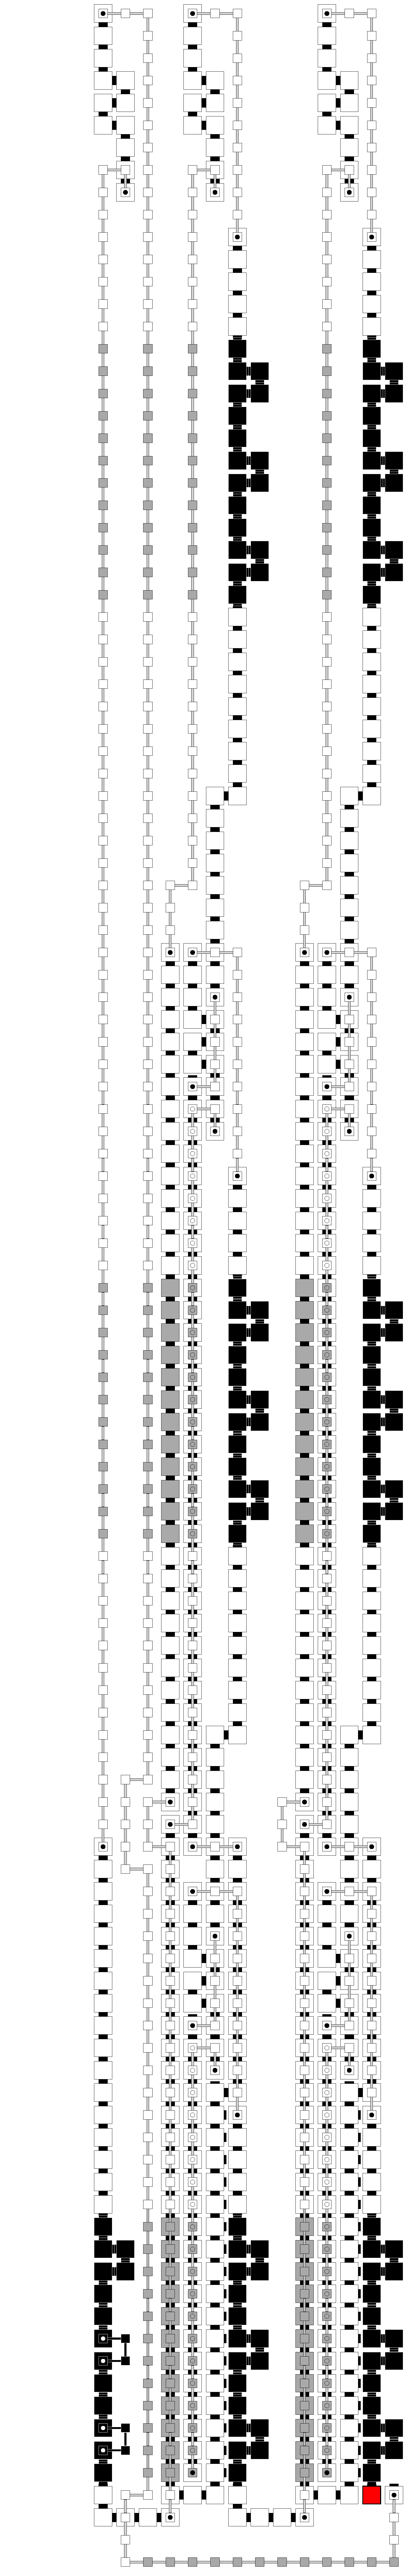
\includegraphics[width=0.95in]{initial_value_overview_case1}}\hfill%
    \subcaptionbox{Initial value case 2\label{fig:initial_value_case2}}{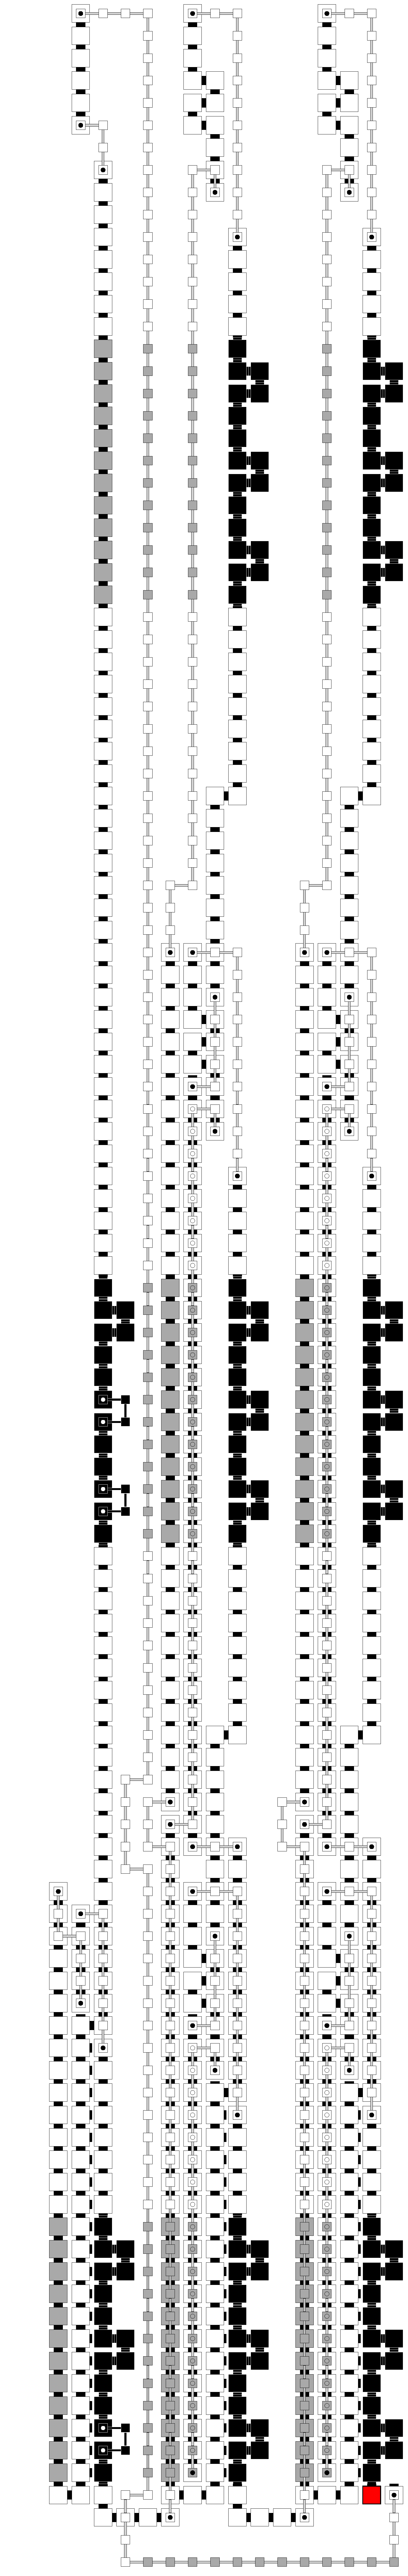
\includegraphics[width=0.95in]{initial_value_overview_case2}}\hfill%
    \subcaptionbox{Initial value case 3\label{fig:initial_value_case3}}{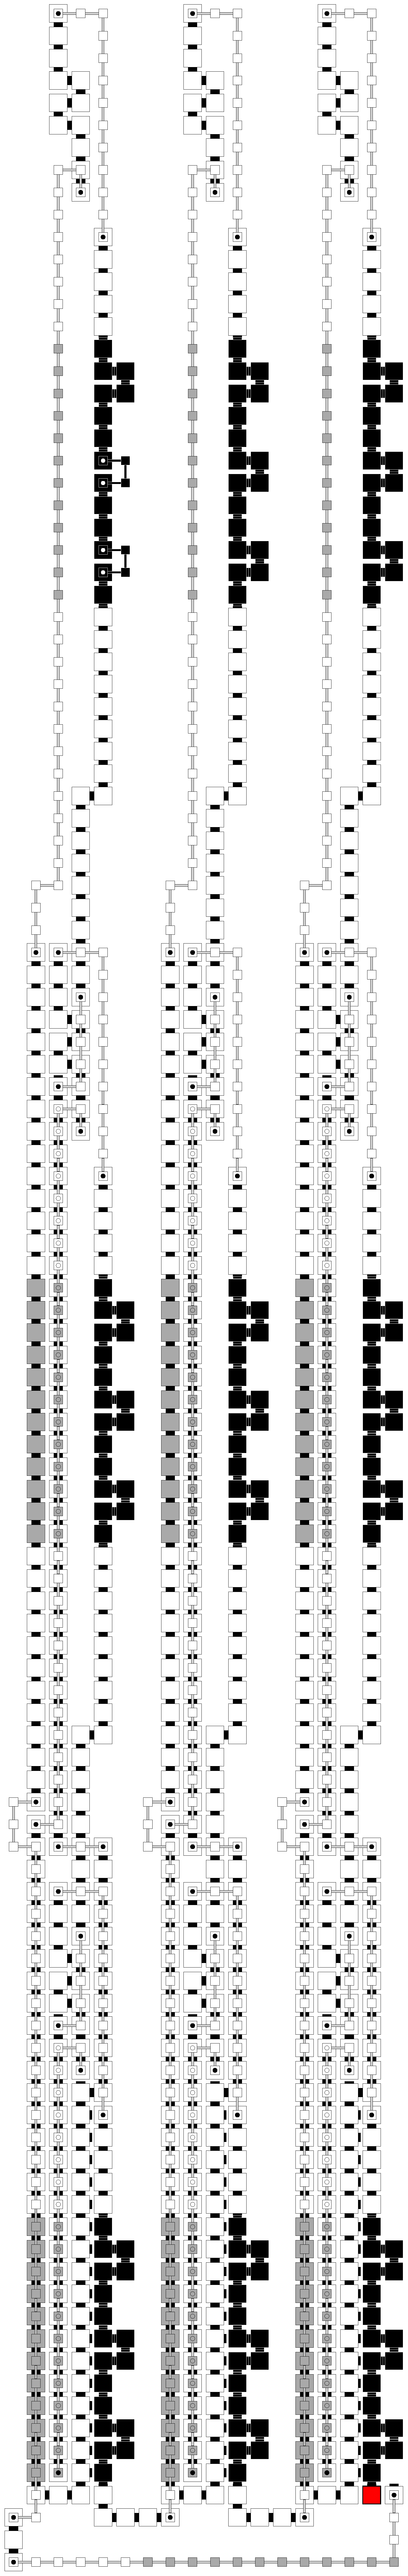
\includegraphics[width=0.95in]{initial_value_overview_case3}}%
    \caption{\label{fig:initial_value_assemblies_full} These figures show a
    full example of an initial value, with both general regions and
    the MSRs together, instead of separated as shown above.}
\end{figure}